\section{Introduction}


% \begin{figure}
% 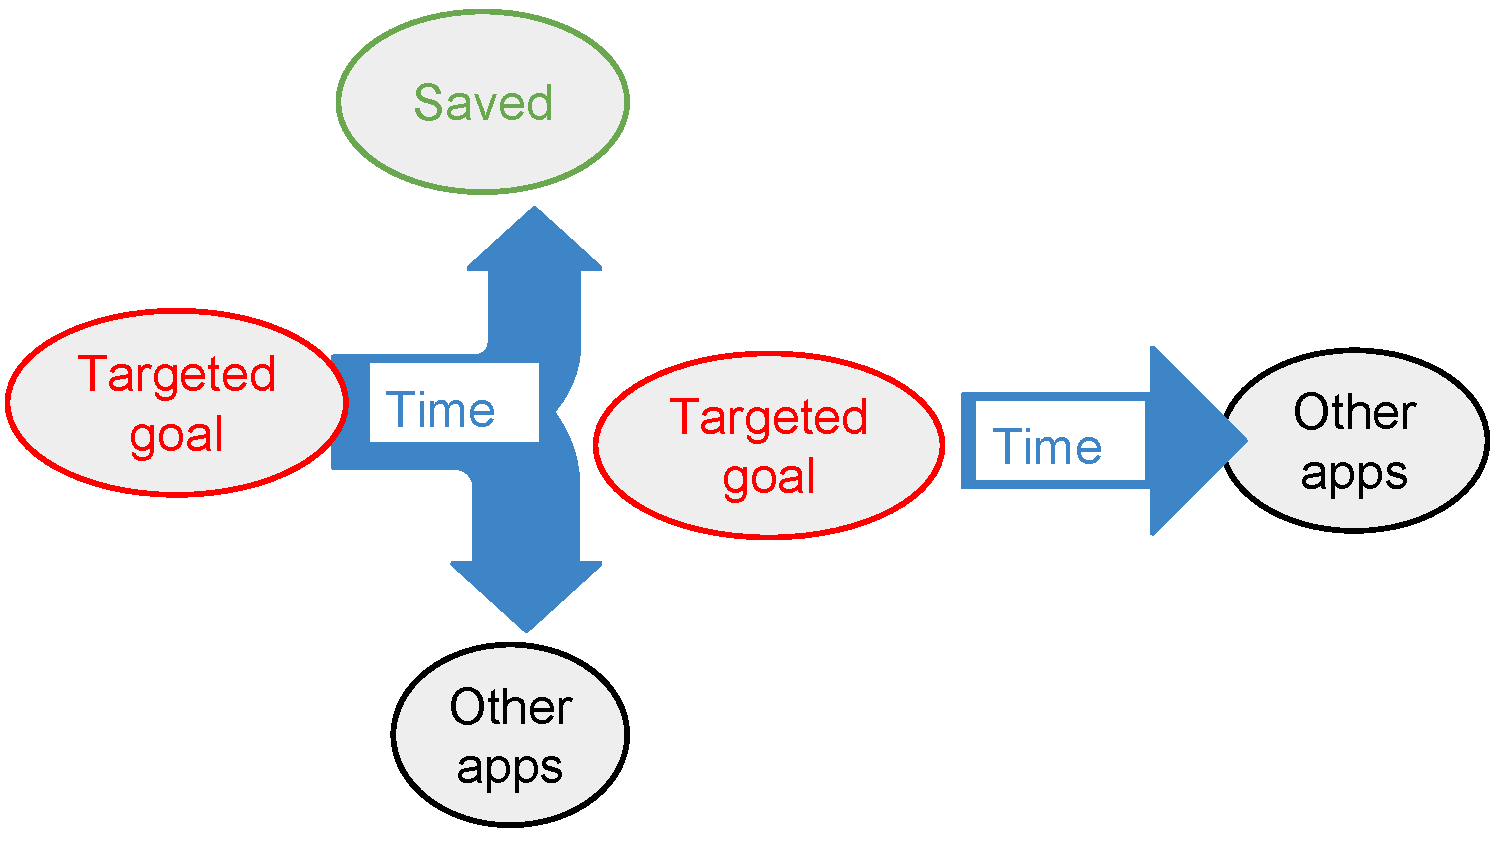
\includegraphics[width=\linewidth]{figures/intro/p01.pdf}
% \caption{}
%   \label{}
% \hfill

% \end{figure}
% \begin{figure}
% 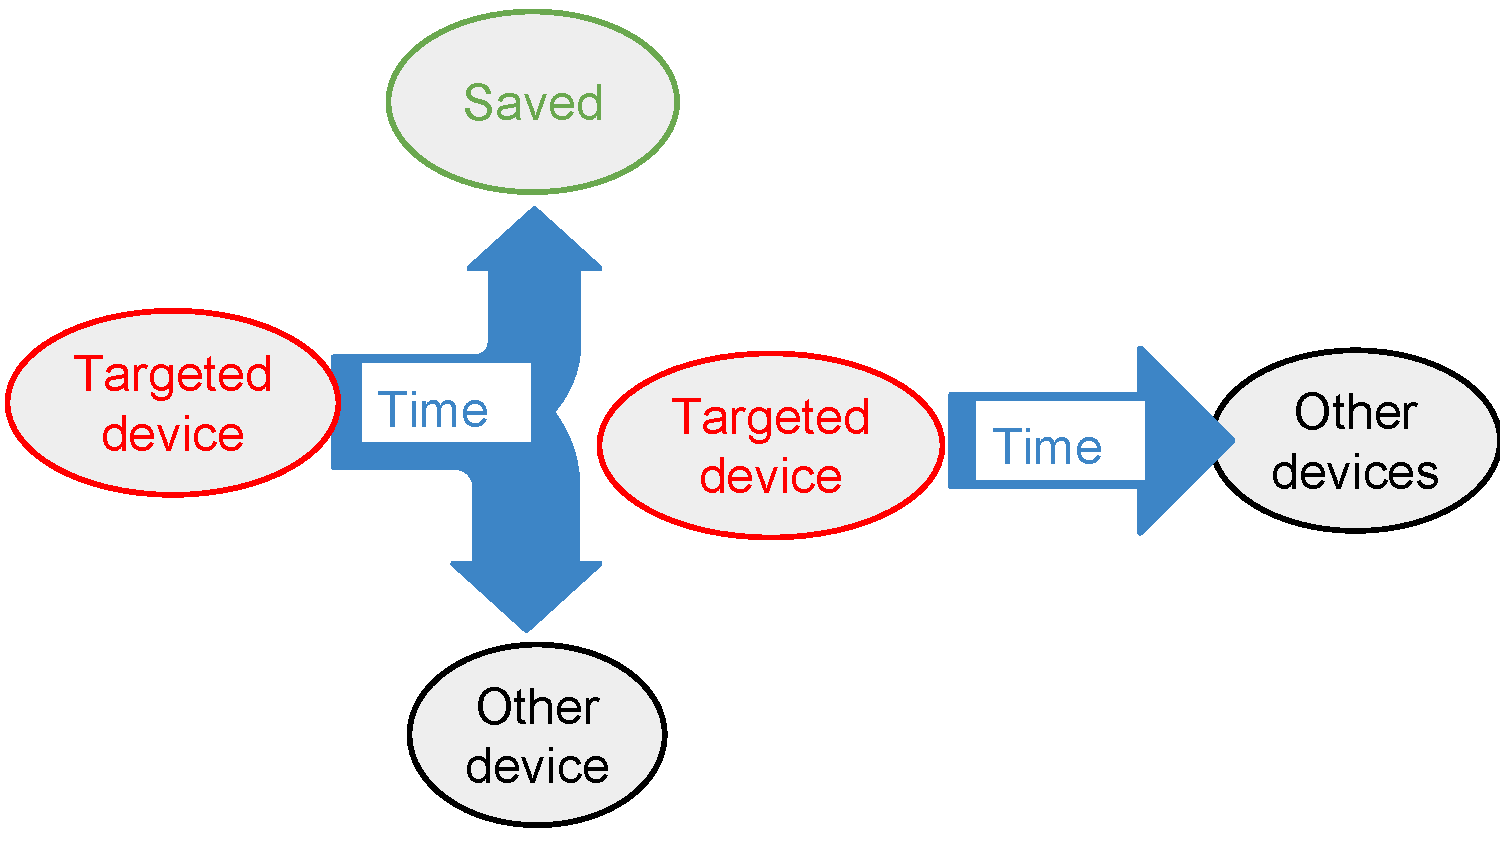
\includegraphics[width=\linewidth]{figures2/intro/p02.pdf}
% \caption{}
%   \label{}
% \hfill

% \end{figure}

% \begin{figure}
% 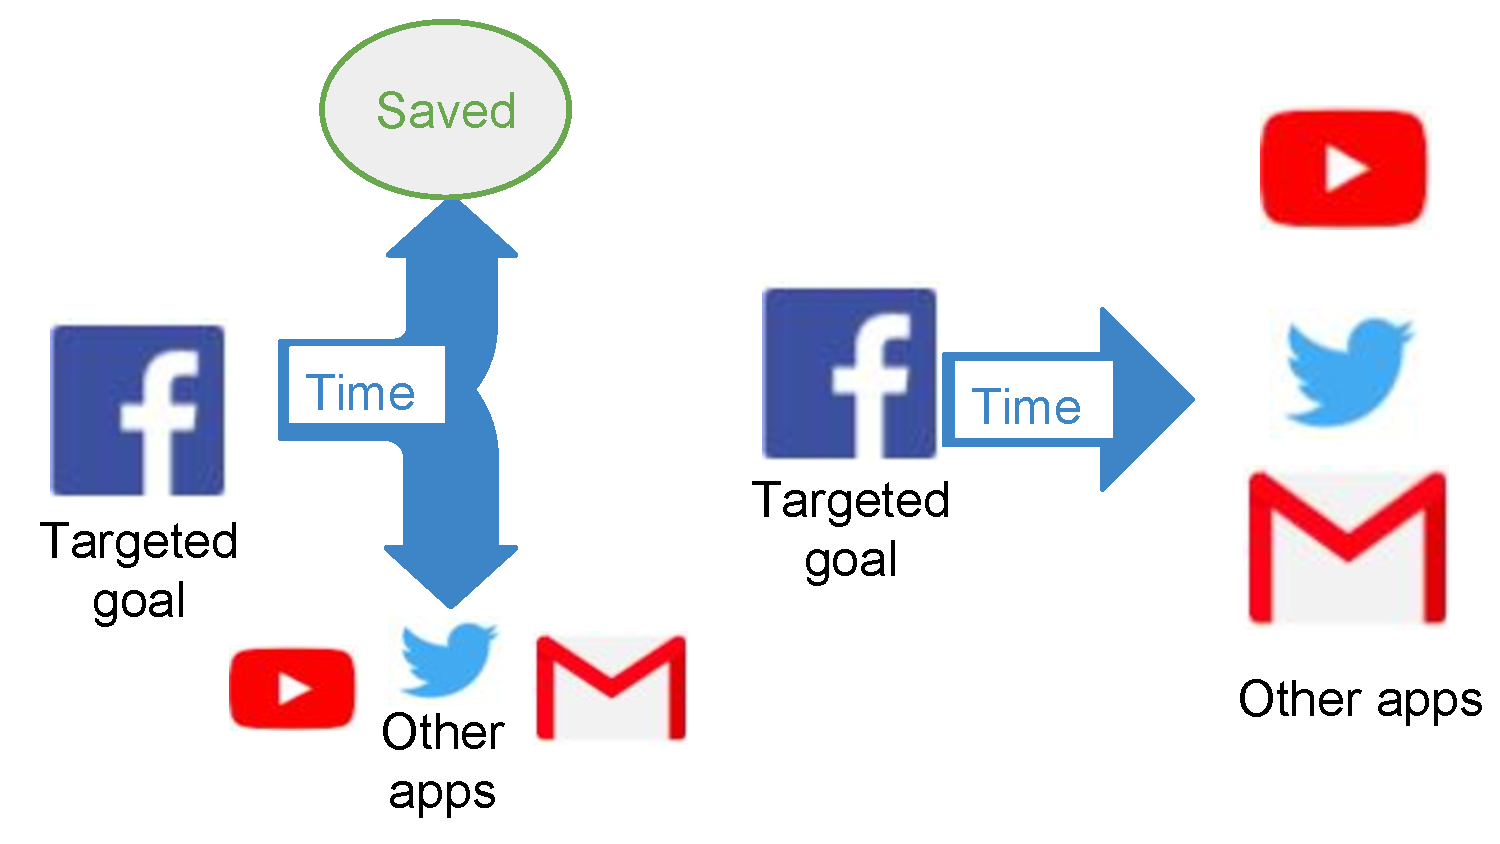
\includegraphics[width=\linewidth]{figures2/intro/p03.pdf}
% \caption{}
%   \label{}  
% \hfill

% \end{figure}
% \begin{figure}
% 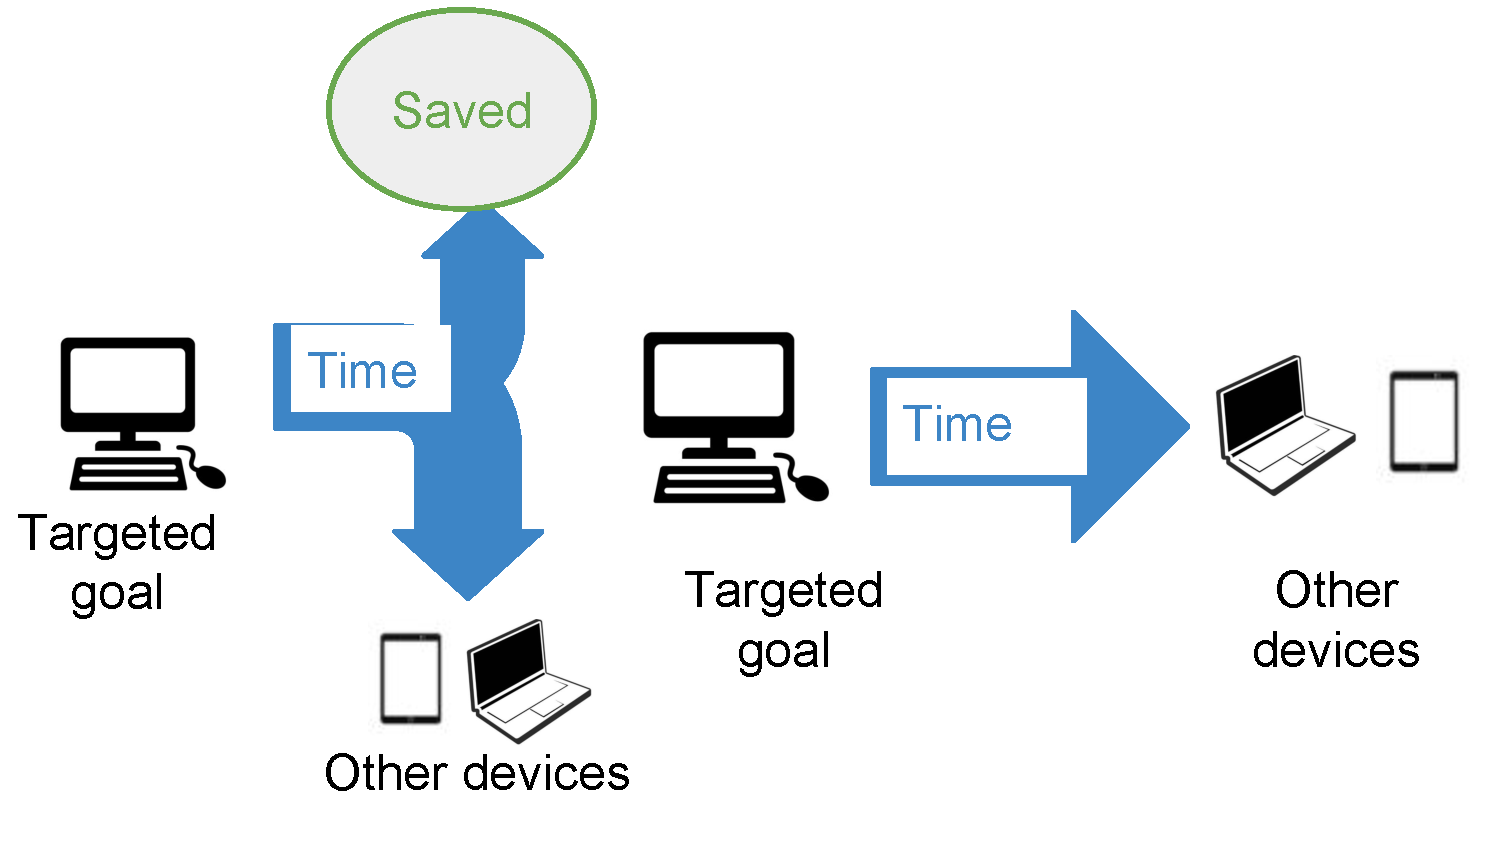
\includegraphics[width=\linewidth]{figures2/intro/p04.pdf}
% \caption{}
%   \label{}
% \hfill

% \end{figure}

\begin{figure}

%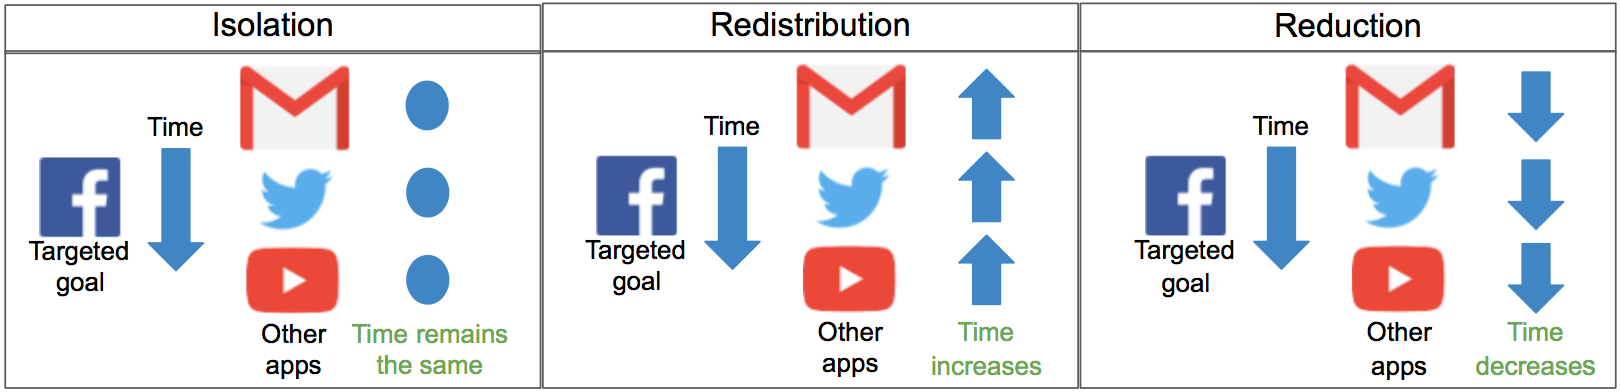
\includegraphics[width=\linewidth, clip,trim=0 0 0.1 0]{figures2/intro/f_1.png}
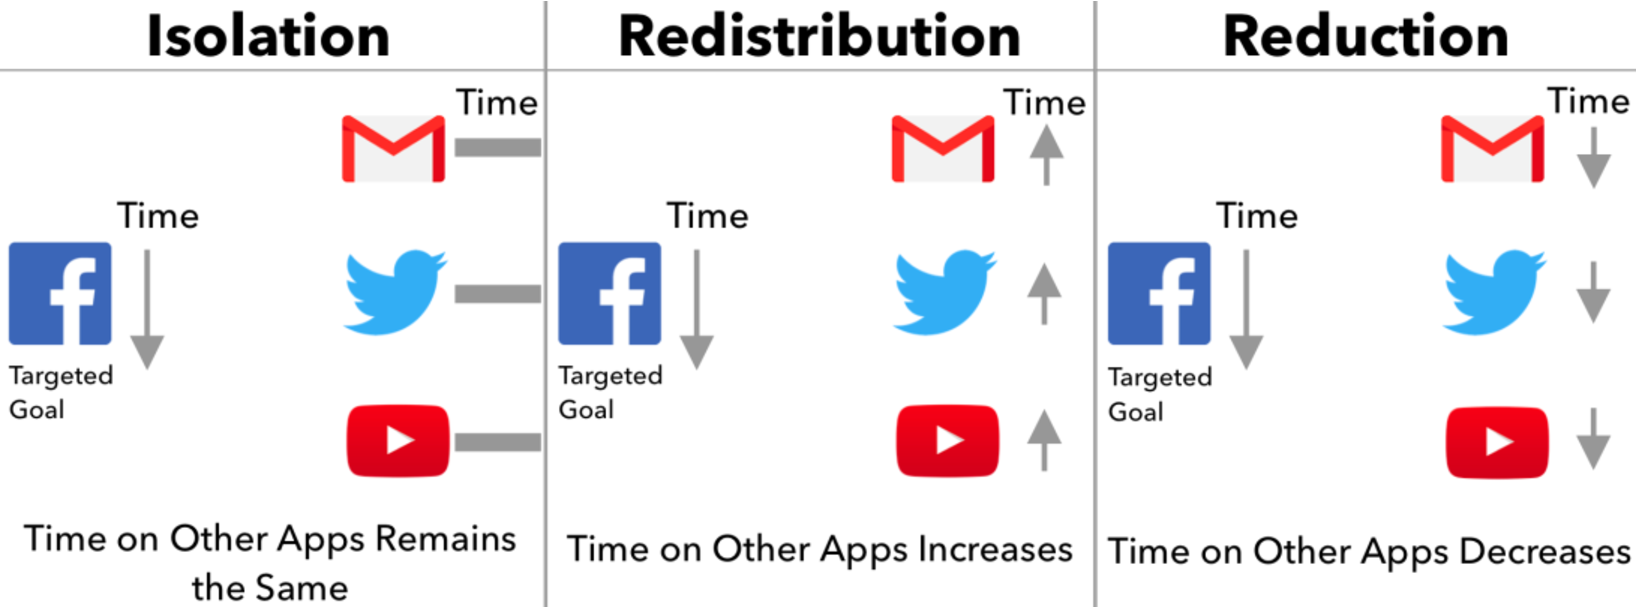
\includegraphics[width=\linewidth, clip,trim=0 0 0.1 0]{figures2/intro/fig1v4.pdf}
\caption{When interventions reduce time on a targeted goal such as Facebook, the time saved may (left)~be isolated from effects on other goals, (center)~be redistributed to other goals, or (right)~decrease time spent on other goals.
%\msb{arrows are too thin, hard to see. fatten 'em up}
%\msb{text is too small to read. don't let it get smaller than the body text of the paper.}
} %\msb{This figure needs to be cleaned up. I see three major goals: first, gestalt grouping and whitespace---things should be close together iff there is meaning in the grouping. For example, arrows should be near the apps that are being affected. Second, use the grid. Right now things are misaligned in many places, like "other apps" vs. "time remains the same". Third, "circle" doesn't convey "no effect" to me. I suggest maybe a dash or flat line? } %\newline
%\goli{Goli: updated figure 1 don't know if it's better or worse}}
%\drew{Drew: I also made a figure (intro/Fig1.pdf) with more space. See which of the three you prefer}

  \label{fig:hypotheses-within}
\end{figure}

\begin{figure}

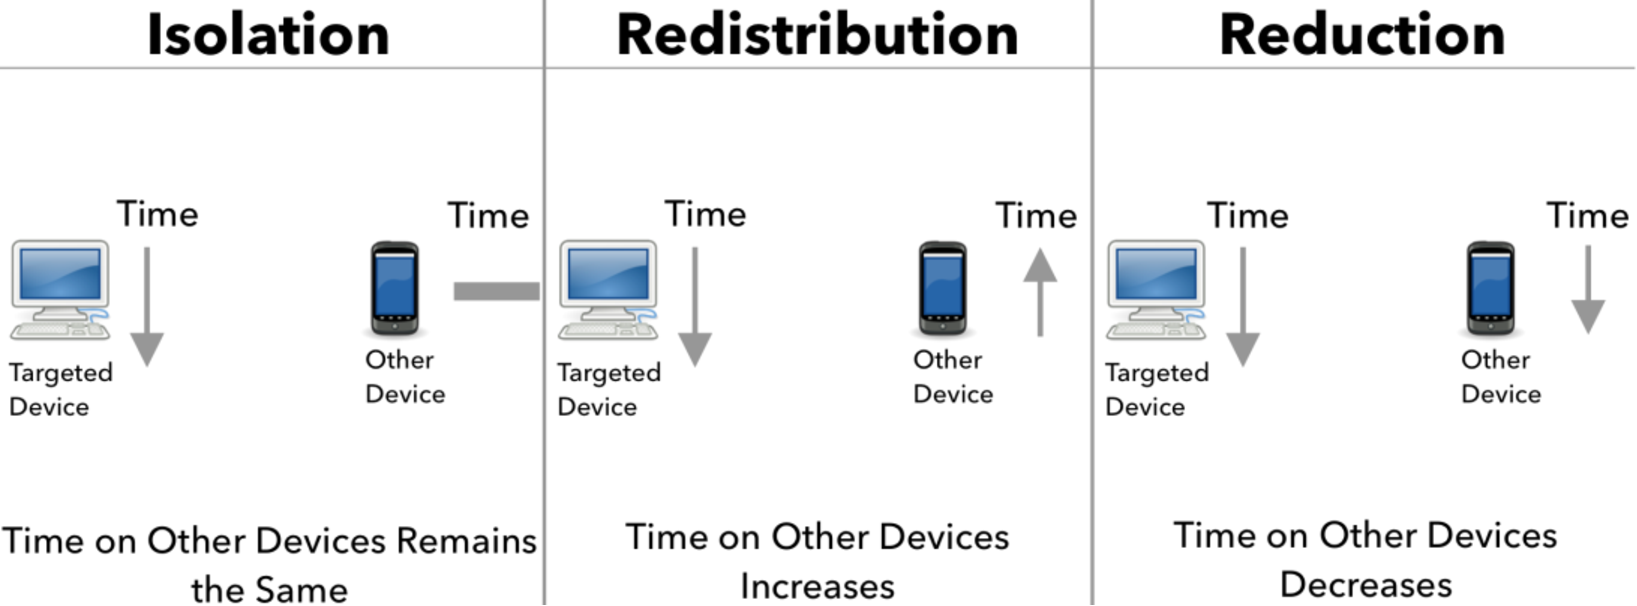
\includegraphics[width=\linewidth]{figures2/intro/fig2v5.pdf}
\caption{When interventions reduce time on a targeted device e.g. a browser, the time saved may (left) be isolated from effects on other devices, (center) be redistributed to other devices, or (right) decrease time spent on other devices.} %platforms similarly to Figure~\ref{fig:hypotheses-within}.
%\msb{arrows are too thin, hard to see. fatten 'em up}
%\msb{text is too small to read. don't let it get smaller than the body text of the paper.}
%}
  \label{fig:hypotheses-across}
\end{figure}

We use productivity behavior change interventions to try to keep ourselves in focus. But do these systems truly save us time? Or do they just redistribute the time elsewhere? In other behavior change domains, interventions sometimes have effects on behaviors other than the ones they were targeting~\cite{stamford1986effects, COTTER2014243}. %There are arguments we can make for several different options.

One possibility is that interventions narrowly impact just the goal that they target, and have no effect on time spent elsewhere. We will refer to this as the \textit{isolated effects hypothesis}. Taking the relationship between time spent on Facebook and Instagram as an example, the isolated effects hypothesis would predict that an intervention that helps reduce time on Facebook should have no effect on time spent on Instagram. Persuasive systems often claim to result in the intended behavioral changes without observable consequences elsewhere, lending support for this hypothesis~\cite{doi:10.1080/15228830802094429,cugelman2013gamification, lyons2014behavior,anderson2013steering, anderson2014engaging}. If the isolated effects hypothesis is true, overall productivity can be boosted through interventions that individually target each goal. %\msb{This paragraph needs grounding through citations in other literature suggesting that it might be the case. Otherwise it's just us handwaving. For example, do we know that smoking cessation interventions don't cause eating problems? The next two paragraphs have a few citations to bolster their case---better examples} %There have been many studies showing that various productivity techniques are effective, so we would hope that overall productivity can be boosted.

However, people have a limited supply of willpower~\cite{baumeister1998ego}, can maintain focus for only so long~\cite{jin2009self,dabbish2011keep,mark2016email}, and need downtime --- so perhaps the time saved is actually just redistributed to other unproductive applications. We will refer to this as the \textit{redistribution hypothesis}: saving time on one unproductive application results in an increase in time spent on other unproductive applications. Returning to our example of a productivity intervention targeting Facebook, redistribution would hypothesize that an intervention that reduces time on Facebook will increase time spent on Instagram.
Redistribution may be partial, where the time redistributed is some fraction of what was saved. Or more bleakly, redistribution may be total, where the time redistributed is entirely shifted to other applications and there is no overall improvement in productivity.
%Within this, there is the possibility for \textit{partial redistribution}, where the amount of time saved in the app/site targeted by the productivity intervention exceeds the amount that is redistributed to other unproductive apps/sites, so overall productivity is still improved, but not as much as we would expect by measuring the effect on the app/site in isolation. A bleaker possibility is \textit{total redistribution}, where amount of time redistributed to other apps equals the time saved on the app targeted by the productivity intervention, so there is overall no improvement in productivity.

A third possibility is that saving time on one application breaks a habit loop~\cite{duhigg2012power} and reduces time spent on other applications as well, so the actual net improvement in productivity is even better than just what is saved on the target application. We will refer to this as the \textit{reduction hypothesis}. Returning to our example of a productivity intervention targeting Facebook, this would hypothesize that an intervention that reduces time on Facebook will also reduce time on Instagram. Perhaps once we enter ``procrastination mode'' and visit one unproductive application, we wind up chaining together visits to another unproductive application, and another---but if a productivity intervention helps us break the chain early on, we will never visit the later unproductive applications.

% Another possibility is a combination of both effects, where overall time is saved but some time is still redistributed to other sources. A third possibility is a symbiotic effect, where 

These three hypotheses lay out the three possibilities of what happens to other goals when we intervene on a focal goal (Figures~\ref{fig:hypotheses-within}--\ref{fig:hypotheses-across}): time on those other goals might stay the same (isolated effects), go up (redistribution), or go down (reduction). In this chapter, we seek to adjudicate between these hypotheses using  HabitLab~\cite{habitlab}, an in-the-wild productivity experimentation environment that users can voluntarily participate in by installing. Prior work described HabitLab as a Chrome browser extension; in this chapter we created and deployed a companion HabitLab Android application, allowing us to study any redistribution of time that might be happening across devices, as when a user avoids Facebook on their browser but ends up checking Facebook on their phone instead.

After installing and agreeing to our experimental protocol, users specify what they wish to reduce time on, which we term \emph{goals}. In the case of the Android version, goals take the form of applications (apps), whereas on the Chrome extension goals are sites.
We then deploy interventions to help users reduce their time on these goals, which can appear when the user visits a website (Chrome) or app (Android). To study redistribution, we periodically manipulate  the frequency at which interventions appear for each goal --- if the goal is in the frequent condition that week, it will appear every time the user visits that application, whereas if the goal is in the infrequent condition that week, it will appear on 20\% of visits. This experimental design allows us to observe the effects of a goal being in the \textit{frequent} setting not only on how much time users spend on that focal goal, but also what happens to time on other goals when that focal goal is in the frequent setting.

% frequency browser 313 -> 288; mobile 375 -> 235; intensity:browser 978 -> 861; android 3450 -> 3075; within platform browser 3667 -> 3096

Our analysis first begins by seeing whether interventions are effective at reducing time on the focal goal, disregarding any possible redistribution effects. We do so by comparing time spent per day on the application on weeks where interventions are shown frequently, vs those weeks where interventions are shown infrequently. We find that they are effective, with time spent on goal sites reduced by 8.0\% on the Chrome version, and time spent on goal apps reduced by 37.3\% on the Android version.

Next, we investigate whether time is redistributed to other sites/apps on the same platform (browser or mobile) when interventions are frequently shown. We find that giving interventions within the browser produces a reduction effect, with users using sites/apps less when there are more interventions shown on other sites/apps -- however, effects of interventions are isolated on mobile. %\msb{out of date? isolation on one platform, reduction on the other}

Finally, we investigate whether time is redistributed across devices. We do not observe any significant time redistribution effects in either direction.

%Finally, we investigate whether time is redistributed across devices. We find that there is an insignificant trend suggesting an increase in time spent on the browser when a user is given interventions more frequently on Android. \msb{is this up to date?}

This chapter contributes a look into potential unintended side effects of productivity interventions on other sites, apps, and devices. We find that productivity interventions do not appear to have deleterious second-order effects on goals other than the ones they are targeting, and in some cases, may even have beneficial second-order effects by breaking habit loops.
%can sometimes have beneficial effects outside the goals they were targeting. %finding that while in some instances there appears to be redistribution, thankfully, it is not a zero-sum game, and there is evidence for global reduction effects.

